\documentclass[aspectratio=169, usenames, dvipsnames]{beamer}

\usetheme{Pittsburgh}

\usepackage[utf8]{inputenc}
\usepackage[german]{babel}
\usepackage{amsmath}
\usepackage{amsfonts}
\usepackage{amssymb}
\usepackage{upgreek}
\usepackage{graphicx}
\usepackage{multicol}
\usepackage{wrapfig}
\usepackage{hyperref}
\usepackage{framed}
\usepackage{lmodern}% http://ctan.org/pkg/lm
\usepackage{anyfontsize}
\usepackage{tikz}
\usetikzlibrary{shapes,arrows}
\usepackage{xspace}                     % Correct spacings
\usepackage{csquotes} 

\author{Jonas Betzendahl}
\title{Formalising and Proving with Sudokus}

\beamertemplatenavigationsymbolsempty 
\setbeamertemplate{footline}[frame number]

\newcommand{\IMPS}{\texttt{IMPS}\xspace}
\newcommand{\MMT}{\textsf{MMT}\xspace}
\newcommand{\LUTINS}{\textsc{LUTINS}\xspace}
\newcommand{\OMDOC}{\textsf{OMDoc}\xspace}
\newcommand{\LF}{\textsf{\textbf{LF}}\xspace}
\newcommand{\LFX}{\textsf{\textbf{LF+X}}\xspace}
\newcommand{\LPL}{$\uplambda$Prolog\xspace}
\newcommand{\ELPI}{\textsf{ELPI}\xspace}

\newcommand{\defined}[1]{{#1}\mkern-5mu\downarrow}
\newcommand{\undefined}[1]{{#1}\mkern-5mu\uparrow}

\begin{document}

%------------------------------------------------------------------------------------
\begin{frame}
\begin{center}
\Large \textbf{Formalising and Proving with Sudokus}

\normalsize 
\bigskip\bigskip

\large Jonas Betzendahl\\
\texttt{jonas.betzendahl@fau.de}\bigskip

\small
WuV-Seminar\\
2021 -- 06 -- 24
\medskip


\includegraphics[scale=0.25]{images/fau_logo.png}
\quad

\includegraphics[scale=0.25]{images/kwarclogo_faublau.png} 
\end{center}
\end{frame}

\section{Introduction}

\begin{frame}
\frametitle{Motivation}

My current research question are \emph{generated} theorem provers for \MMT theories.
\bigskip

The idea being that a user could formalise whatever theory they needed, could then press a button and get a program that can solve some proof obligations for them, using the rules of their new theory.
\bigskip

Nobody expects these provers to produce mathematically interesting insights or prove big theorems, but
if we can take the busywork off the user's hands, that's already very helpful.
\end{frame}

\begin{frame}
\frametitle{Test Cases}
I anticipate the most use for these provers for simple proof obligations to be in the field of Undefinedness and Soft Types, two other topics of my PhD program.
\medskip

Both of these have a tendency to generate loads of tiny obligations that would be prohibitively tedious to prove yourself all the time. Tests in the realm of Propositional Logic have been successfull.
\bigskip\pause

Hence, I thought that solving Sudokus (well-known, easy to conceptualise and famously NP-complete [in the generalised case]) might make a good case study.

This talk is about what I found out. 
\end{frame}

\section{Sudoku}

\begin{frame}
\Huge
\begin{center}
Sudoku\large\\
---------------------\\
The game, the strategies and my formalisation.
\end{center}
\end{frame}

\begin{frame}
\frametitle{The Game of Sudoku}
\begin{minipage}{0.45\textwidth}
\begin{center}
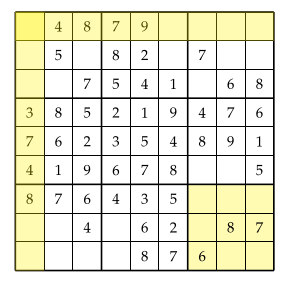
\includegraphics[height=0.70\textheight,keepaspectratio]{images/sudoku_blank} 
\end{center}
\end{minipage}
\begin{minipage}{0.475\textwidth}
Sudoku (jpn.: ``Single Number'') is a popular logic-based, combinatorial number puzzle.
\bigskip
\begin{itemize}
\item 81 \emph{cells} arranged in (partially filled) square grid.
\item Rows, Colums and 3x3 Boxes form connected \emph{houses}.
\item In a solution, each house needs to contain each digit ($1-9$) exactly once.
\end{itemize}
\end{minipage}

\end{frame}

\begin{frame}
\frametitle{Pencil Marks}

A common approach for both humans and computers trying to solve Sudokus is to keep track of which digits could possibly or need to be necessarily filled into which cells with so-called \emph{Pencil Marks}.

\begin{center}
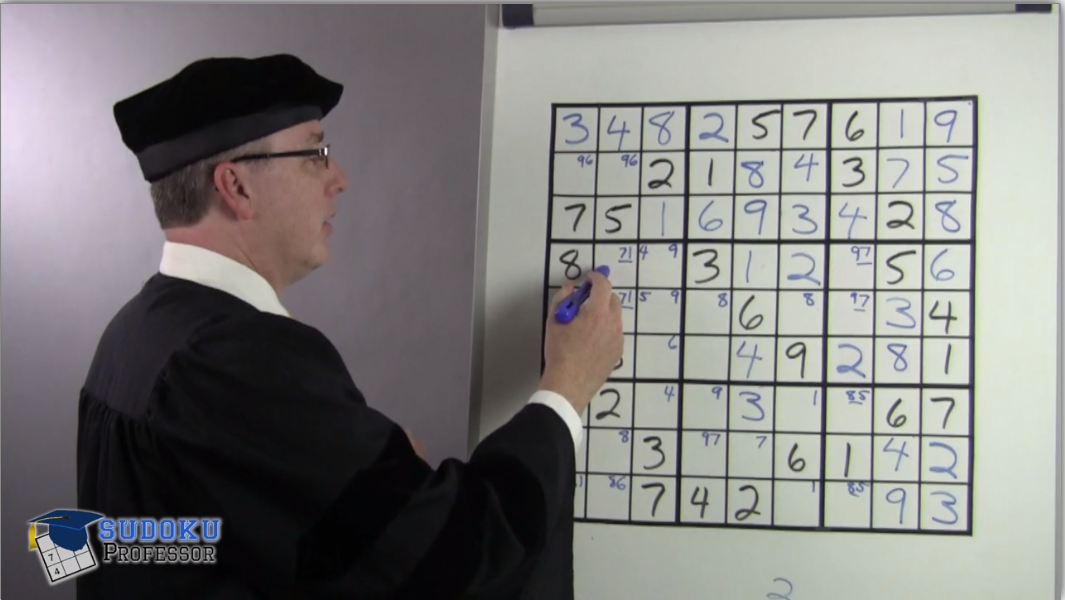
\includegraphics[height=0.5\textheight, keepaspectratio]{images/professor_pencil_mark.png} 
\end{center}
\end{frame}

\begin{frame}
\frametitle{Formalisation (1): Kripke Models}
The \emph{possibility} and \emph{necessity} of digits being filled into cells being such a central element to the puzzle makes applying \emph{Modal Logic} an obvious choice. We will be following Daan Di Scala's formalisation of Sudoku as a Kripke Model\footnote{Available at: \url{http://dspace.library.uu.nl/handle/1874/396282}}.

\begin{center}
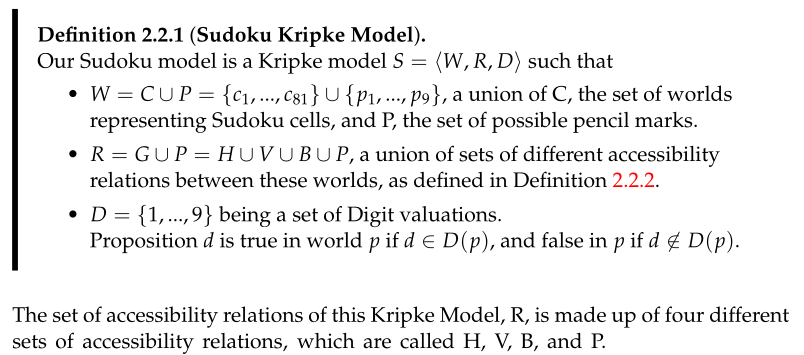
\includegraphics[scale=0.35]{images/kripke_model.png} 
\end{center}
\end{frame}

\begin{frame}
\frametitle{Formalisation (2): Modal Logic}
In this framework, we have $81 + 9 = 90$ worlds and ``Solving the Sudoku'' means reasoning about the accessibility relations until each cell-world has access to exactly one digit-world.
\bigskip

In the following, these notations will be used:
\medskip

\begin{center}
\begin{tabular}{ c | l }
  $c_x \; B \; c_y$ & $c_x$ and $c_y$ are in the same block\\
  $S, c_x \vDash \square_V \varphi$ & $\varphi$ is the case in all cells in the same column.\\
  $S, c_{21} \vDash \square_p (3 \otimes 5)$ & Cell $c_{21}$ necessarily contains either a $3$/$5$.\\
  $S, c_{81} \vDash \square_H (\diamond_p 6 \wedge \diamond_p 8)$ & Cells hor. reachable from cell $c_{81}$ possibly contain a $6$/$8$.
\end{tabular}
\end{center}

Reasoning will happen inside a ND calculus.
\end{frame}

\begin{frame}
\frametitle{Formalisation (3): House Relations}
\begin{minipage}{0.52\textwidth}
\begin{center}
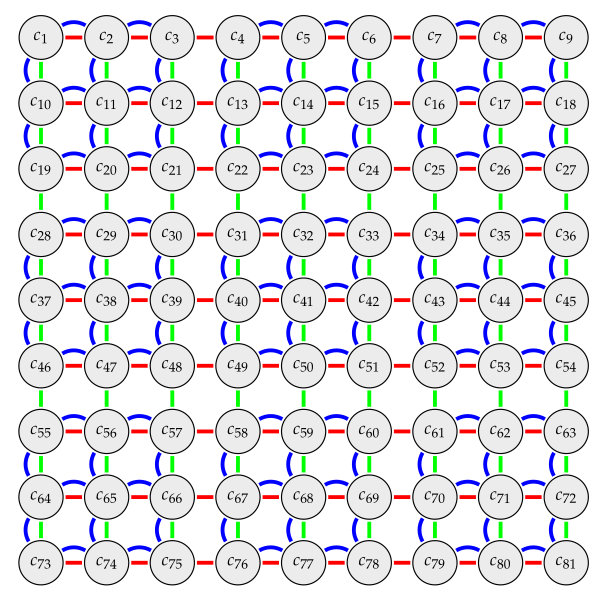
\includegraphics[height=0.75\textheight,keepaspectratio]{images/house_relations.png} 
\end{center}
\end{minipage}\begin{minipage}{0.41\textwidth}
There are three house relations:
\begin{itemize}
\item Same Row
\item Same Column
\item Same Box
\end{itemize}
\bigskip

These are symmetric and transitive but (at least in this writeup) not reflexive.
\medskip

They are realised through (an avalanche of) single constants stating the connection as axioms.
\end{minipage}

\end{frame}

\begin{frame}
\frametitle{Formalisation (4): Helpers}
The formalisation of the Sudoku puzzle itself is relatively straightforward. However, 
to reasonably talk about the rules of the game, it is often necessary to implement
helpers like this one.

As you can see, these can become quite unwieldy.

\begin{center}
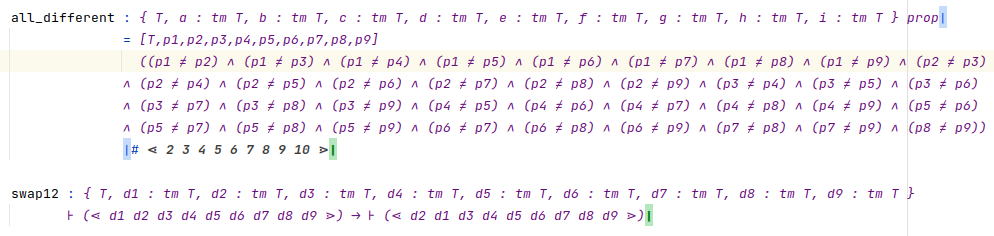
\includegraphics[scale=0.39]{images/helpers.png} 
\end{center}
\end{frame}

\section{Sudoku Strategies}

\subsection{CBE}
\begin{frame}
\frametitle{Strategy 1: Cell-Based Elimination}
\begin{center}
\emph{``If a cell already contains a certain digit, it cannot contain another digit''}
\bigskip

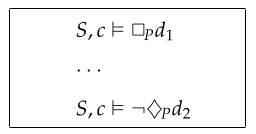
\includegraphics[scale=0.5]{images/strategy_nd_cbe.png} 
\end{center}
\end{frame}

\begin{frame}
\frametitle{Formalising Strategy 1}
\begin{center}
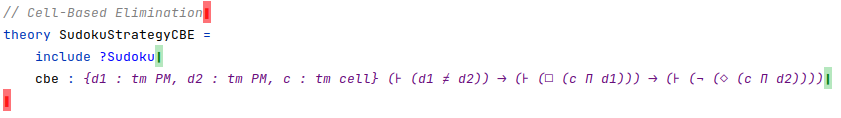
\includegraphics[width=\textwidth, keepaspectratio]{images/strategy_form_cbe.png} 
\pause\bigskip

Straightforward and easy to write down. :)
\end{center}
\end{frame}

\subsection{PMD}
\begin{frame}
\frametitle{Strategy 2: Pencil-Mark Duality}
\begin{center}
\emph{``[W]ith a total of $n$ digits, if in a certain cell there are $m$ PMs possible and $n-m$ PMs not possible, this means that the digit to fill in must be [one] of the $m$ Pencil Marks''}
\bigskip

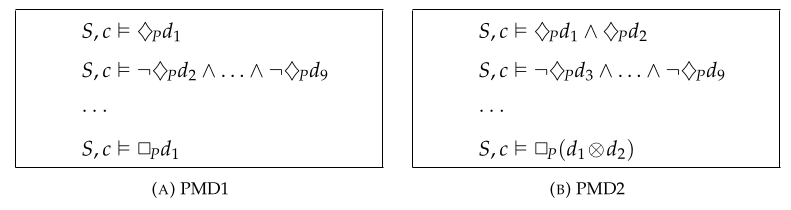
\includegraphics[height=0.4\textheight,keepaspectratio]{images/strategy_nd_pmd.png} 
\end{center}

\end{frame}

\begin{frame}
\frametitle{Formalising Strategy 2}
\begin{center}
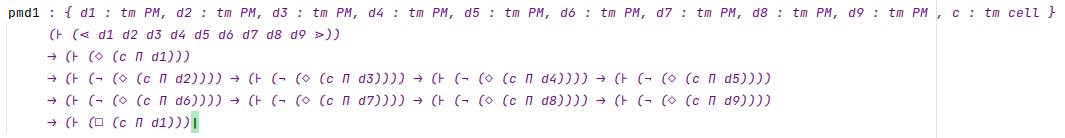
\includegraphics[width=\textwidth, keepaspectratio]{images/strategy_form_pmd.png}
\pause\bigskip

This one is a little more difficult.\\
Also, this is showing only one of many instances of this rule.
\end{center}
\end{frame}

\subsection{HBE}

\begin{frame}
\frametitle{Strategy 3: House-Based Elimination}
\begin{center}
\emph{``If a cell in a house already contains a digit, another cell\\ in the same house cannot contain the same digit''}
\bigskip

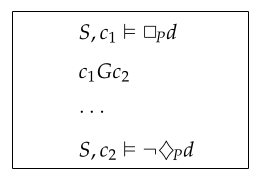
\includegraphics[height=0.4\textheight,keepaspectratio]{images/strategy_nd_hbe.png} 
\end{center}

\end{frame}

\begin{frame}
\frametitle{Formalising Strategy 3}
\begin{center}
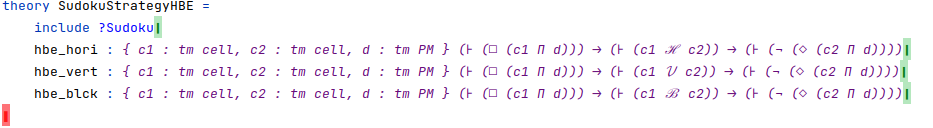
\includegraphics[width=\textwidth, keepaspectratio]{images/strategy_form_hbe.png}
\pause\bigskip

Multiple rules needed, but not too bad.\\
This would be fine if all rules were like this.
\end{center}
\end{frame}

\subsection{LRC}

\begin{frame}
\frametitle{Strategy 4: Last Remaining Cell}
\begin{center}
\emph{``If all the other cells in the same house cannot possibly contain a certain digit,\\ then this cell must contain that digit''}
\bigskip

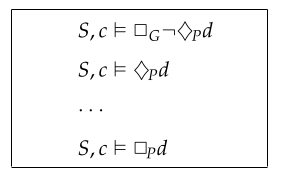
\includegraphics[height=0.4\textheight,keepaspectratio]{images/strategy_nd_lrc.png} 
\end{center}

\end{frame}

\begin{frame}
\frametitle{Formalising Strategy 4}
\begin{center}
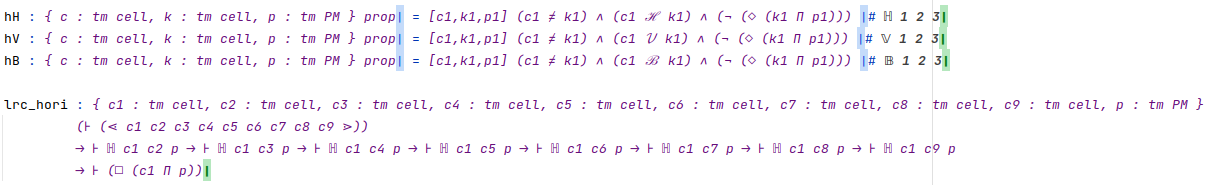
\includegraphics[width=\textwidth, keepaspectratio]{images/strategy_form_lrc.png}
\pause\bigskip

Pretty bad. Three helper constants and still the three rules\\ (only one shown) are getting quite convoluted.
\end{center}
\end{frame}

\subsection{PMI}

\begin{frame}
\frametitle{Strategy 5: Pencil Mark Introduction}
\begin{center}
\emph{``If in none of the three houses of a cell another cell must contain a digit,\\
this cell can possibly contain this digit''}
\bigskip

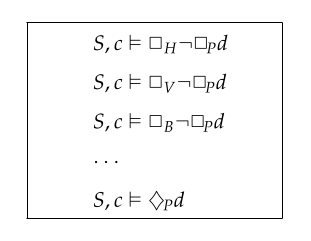
\includegraphics[height=0.4\textheight,keepaspectratio]{images/strategy_nd_pmi.png} 
\end{center}

\end{frame}

\begin{frame}
\frametitle{Formalising Strategy 5}
\begin{center}
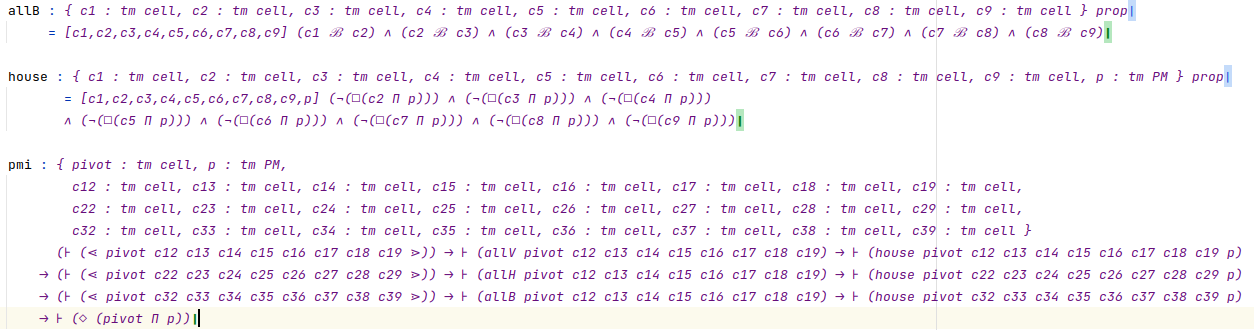
\includegraphics[width=\textwidth, keepaspectratio]{images/strategy_form_pmi.png}
\pause\bigskip

Multiple helpers and still the rule itself is gigantic (26 arguments!).\\
Absolutely terrible for what seems such a basic rule.
\end{center}
\end{frame}

\subsection{Advanced Strategies}

\begin{frame}
\frametitle{Intermediate \& Advanced Strategies}

There are four more strategies on the Intermediate and Advanced Level, quickly rising in complexity.
\bigskip

\begin{center}
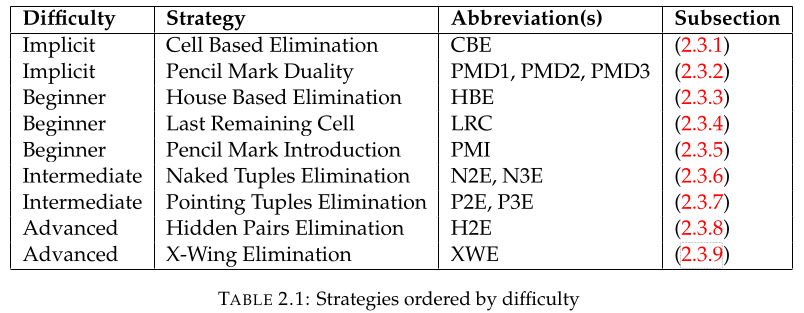
\includegraphics[width=0.8\textwidth, keepaspectratio]{images/all_strategies.png} 
\end{center}

\end{frame}

\begin{frame}
\frametitle{X-Wing Elimination...}

\begin{minipage}{0.45\textwidth}
\begin{center}
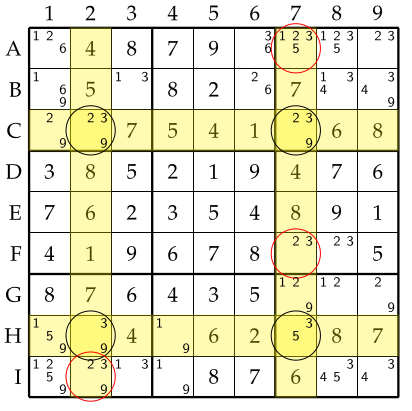
\includegraphics[width=0.8\textwidth, keepaspectratio]{images/xwing.png} 
\end{center}
\end{minipage}\begin{minipage}{0.55\textwidth}
\begin{center}
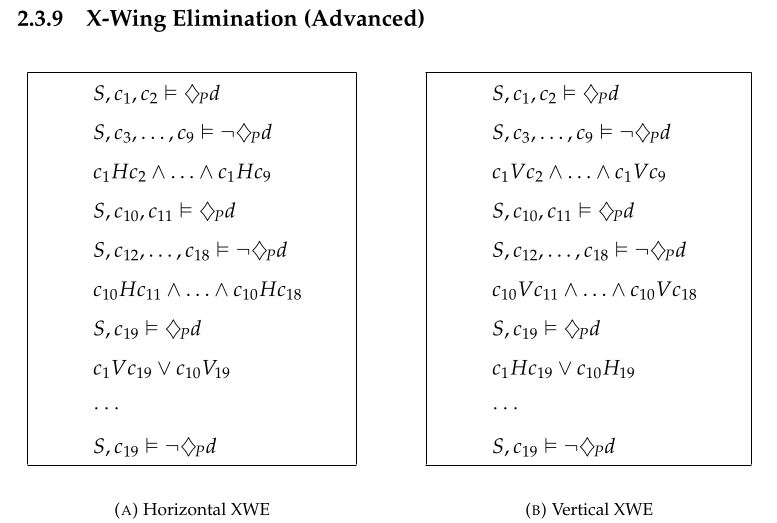
\includegraphics[width=\textwidth, keepaspectratio]{images/strategy_nd_xwing.png} 
\end{center}
\end{minipage}

\pause\bigskip

\begin{center}
\large
\dots not considered. Too complex.
\end{center}
\end{frame}

\section{ELPI Provers}

\begin{frame}
\Huge
\begin{center}
\ELPI \& Provers\large\\
---------------------\\
Prolog for proving
\end{center}
\end{frame}

\begin{frame}
\frametitle{What is ELPI?}
\LPL is a programming language based on an intuitionistic fragment of Church's Simple Theory of Types that extends Prolog by features such as abstract data types and higher-order programming, adding Harrop Formulas to Prolog's underlying foundation of Horn clauses.
\medskip

\LPL is interesting for our problem since we can use its higher-order unification algorithm for proof search.
\pause\bigskip

The \ELPI system is an implementation of \LPL with additional features and a focus on performance, moving some previously intractable proof searches into reach. It is implemented in the OCaml programming language.

\end{frame}

\begin{frame}
\frametitle{The Generated Provers}
I am picking up on previous work by Cohen, Rabe and Schaefer. For any given \MMT theory, one can generate an \ELPI \emph{kernel}, a file that introduces the declarations of a theory and \ELPI rules that reflect the inference rules of the theory (e.g. $\wedge_I$ or $\neg_E$).
\pause\bigskip

One also generates \emph{experts}, i.e. \ELPI modules that apply strategies and/or apply help predicates to reduce the enormous search space of proof terms that would otherwise be intractable.
\end{frame}

\begin{frame}
\frametitle{Proof Certificates}
The behaviour and the output of these \ELPI provers can be guided by the user through selection of so-called ``Proof Certificates''.
\bigskip

These can be the simple difference between a straightforward iterative deepening proof or the more sophisticated backchaining proof where certain rules are only applied under certain circumstances (to manage search space).
\pause\bigskip

They can also deliver an actual proof certificates (compare Dale Miller's \textsf{ProofCert} project\footnote{See: \url{http://www.lix.polytechnique.fr/Labo/Dale.Miller/ProofCert/})} which contain a witness of the successful proof. These can become extremely important as they might need to be checked by \MMT at some point (because relying on \ELPI for proofs can introduce trust issues).
\end{frame}

\subsection{Examples}

\begin{frame}
\frametitle{Example Provers (1)}
Here's a snippet of a generated prover for a rule for negation elimination:
\begin{center}
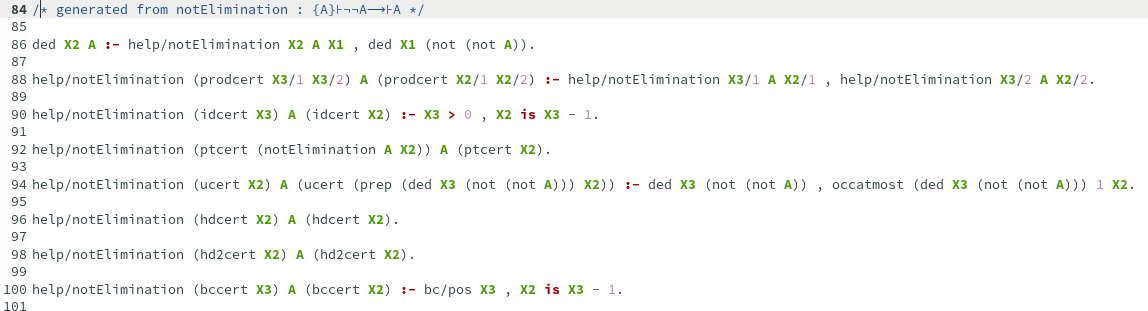
\includegraphics[width=\textwidth, keepaspectratio]{images/plnd_generated.png} 
\end{center}
\end{frame}

\begin{frame}
\frametitle{Example Provers (2)}
This is how a test-case looks like:
\begin{center}
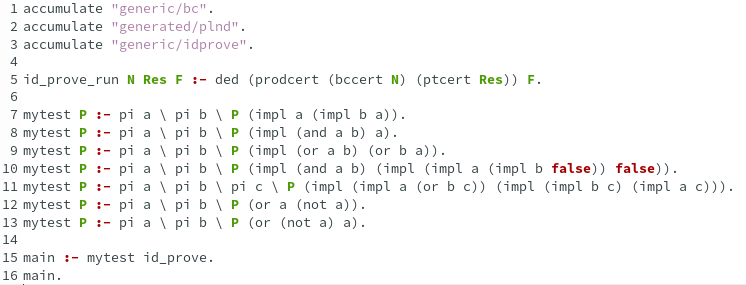
\includegraphics[width=\textwidth, keepaspectratio]{images/plnd_test.png} 
\end{center}
\end{frame}


\begin{frame}
\begin{center}
\Large
live demo...
\end{center}
\end{frame}

\section{Results}

\begin{frame}
\Huge
\begin{center}
Results\large\\
---------------------\\
Does it work as described for Sudokus?
\end{center}
\end{frame}

\begin{frame}
\begin{center}
\Huge
No.
\end{center}
\end{frame}

\begin{frame}
\frametitle{What works?}

Formalisation of Implicit and Beginner Strategies (Di Scala's classification) is complete.
\bigskip\pause

Currently, the generated prover can prove simple facts about a given Sudoku (e.g. $c_i \mathcal{V} c_j$ given that $c_j \mathcal{V} c_i$ and the fact that $\mathcal{V}$ is symmetric).
\bigskip\pause

The prover seems ``stuck'' after only a few layers of iterative deepening, which Frederick and I determined not to be an actual infinite loop, but simply a combinatorial explosion.

\end{frame}

\begin{frame}
\frametitle{What does not?}
Formalisation of Intermediate and Advanced Strategies has not started (no need to waste time on that).
\bigskip\pause

Even the simplest steps (solving a Sudoku from a completely filled board sans one cell) is currently too complicated for generated provers.

\end{frame}

\begin{frame}
\frametitle{Major Problems?}

\begin{itemize}
\item \textbf{\MMT is good for the logic-based part but bad for the combinatorial part}\\
Some preconditions are incredibly complicated to write and require a lot of proving power
\medskip
\item \textbf{The formalisation of modal logic is incomplete}\\
LATIN2 contains the basics but needs more rules and theorems that the provers can use.
\medskip
\item \textbf{Backchaining Algorithm is not up to par for this task}\\
There needs to be a better way of reducing search space.
\end{itemize}

\end{frame}

\section{Outlook}

\begin{frame}
\Huge
\begin{center}
Outlook\large\\
---------------------\\
Where do we go from here?
\end{center}
\end{frame}

\begin{frame}
\frametitle{Plans}
In the short term, I will\dots
\medskip

\begin{itemize}
\item\dots improve the Backchaining algorithm.
\item\dots see if the provers are more helpful with more hand-encoded domain knowledge.
\item\dots focus on test cases with less combinatorial explosion.
\end{itemize}
\pause\bigskip

In the long term, I would like to\dots
\medskip

\begin{itemize}
\item\dots see if I can re-work my formalisation.
\item\dots try to find more ways to easily encode domain knowledge that can be used by provers.
\item\dots revisit Sudokus as a hard test case.
\end{itemize}
\end{frame}

\begin{frame}
\frametitle{Strategy Graph}
\begin{minipage}{0.65\textwidth}
\begin{center}
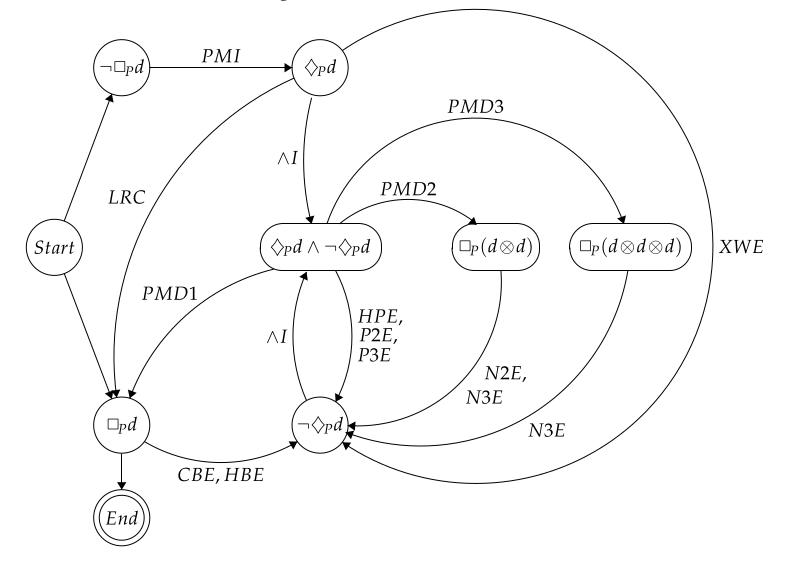
\includegraphics[height=0.7\textheight, keepaspectratio]{images/strategy_graph.png} 
\end{center}
\end{minipage}\begin{minipage}{0.3\textwidth}
We could use the so-called ``Strategy Graph'' from Di Scala's thesis as a way to reduce the search space.
\bigskip

This could also function as a case study for encoding domain knowledge as effectively usable for the provers.
\end{minipage}
\end{frame}

\begin{frame}
\frametitle{Conclusion}

We set out to investigate whether the problem of Sudoku can be solved with the current state of the generated \ELPI provers.
\pause\bigskip

\begin{center}
\emph{I still believe Sudoku is an interesting case study for this problem space!}
\pause

\dots but a lot needs to happen before it becomes feasible.
\end{center}
\bigskip\pause

This experiment has, however clearly demonstrated where the current state's weaknesses are and what needs to be tackled next.
\bigskip\pause

Please feel free to share your Questions, Feedback and Ideas with me now!

\end{frame}

\begin{frame}
\frametitle{Sources}
\vfill
\begin{center}
\url{https://kwarc.info/public/proposal_jbetzendahl.pdf}\\
\url{http://dspace.library.uu.nl/handle/1874/396282}\\
\url{https://gl.mathhub.info/MMT/LATIN2/-/tree/devel/elpi}
\url{https://github.com/LPCIC/elpi}
\bigskip

\emph{Full bibliography available upon request.}
\end{center}
\vfill
\end{frame}

\end{document}